\section{Thiết kế và cài đặt hệ thống gợi ý việc làm}
\label{sec:thiet-ke-he-thong}

\subsection{Kiến trúc tổng thể}
\label{subsec:kien-truc-tong-the}

Hệ thống gợi ý việc làm được thiết kế theo kiến trúc module hóa, trong đó các thành phần được tổ chức thành các module độc lập với trách nhiệm rõ ràng. Hình \ref{fig:system-architecture} minh họa các module chính và mối quan hệ giữa chúng.

Hệ thống bao gồm bốn module chính. Module RecommendationService đóng vai trò điều phối, quản lý toàn bộ quy trình gợi ý từ tải dữ liệu, tính toán embedding, đến lưu kết quả. Module EmbeddingService chịu trách nhiệm chuyển đổi văn bản thành vector nhúng sử dụng mô hình SimCSE. Module SimilarityService thực hiện tìm kiếm tương tự và thuật toán lọc phân tầng thông qua chỉ mục FAISS. Module Repositories cung cấp lớp trừu tượng để truy cập cơ sở dữ liệu PostgreSQL.

Luồng dữ liệu trong hệ thống diễn ra như sau. Đầu tiên, RecommendationService tải danh sách CV và công việc từ Repositories và kiểm tra mã băm nội dung để xác định các bản ghi cần cập nhật. Tiếp theo, EmbeddingService tính toán vector nhúng cho các bản ghi có nội dung thay đổi và lưu kết quả vào PostgreSQL thông qua Repositories. Sau đó, SimilarityService xây dựng hoặc tải chỉ mục FAISS từ các vector tiêu đề công việc và thực hiện thuật toán lọc phân tầng để tìm các công việc phù hợp nhất cho mỗi CV. Cuối cùng, kết quả gợi ý được lưu vào bảng RecommendJobForCV.

\begin{figure}[H]
\centering
\begin{tikzpicture}[
    module/.style={rectangle, draw, fill=blue!15, minimum width=3cm, minimum height=0.8cm, text centered, rounded corners=3pt, font=\small},
    storage/.style={cylinder, draw, fill=gray!20, minimum width=2cm, minimum height=0.8cm, aspect=0.3, font=\small},
    arrow/.style={->, >=stealth, thick},
    dasharrow/.style={->, >=stealth, dashed}
]

% Services layer
\node[module, fill=yellow!20] (recsvc) at (0, 2) {RecommendationService};
\node[module, fill=blue!15] (embedsvc) at (-3.5, 0.5) {EmbeddingService};
\node[module, fill=blue!15] (simsvc) at (3.5, 0.5) {SimilarityService};

% Database layer
\node[module, fill=green!15] (repo) at (0, -1) {Repositories (CV, Job, Recommendation)};

% Storage
\node[storage] (db) at (-3, -2.5) {PostgreSQL};
\node[storage] (faiss) at (3, -2.5) {FAISS Index};

% Arrows
\draw[arrow] (recsvc) -- (embedsvc);
\draw[arrow] (recsvc) -- (simsvc);
\draw[arrow] (recsvc) -- (repo);
\draw[arrow] (embedsvc) -- (repo);
\draw[arrow] (simsvc) -- (faiss);
\draw[arrow] (repo) -- (db);
\draw[dasharrow] (db) -- (faiss) node[midway, below, font=\footnotesize] {build index};

\end{tikzpicture}
\caption{Kiến trúc module hệ thống gợi ý việc làm}
\label{fig:system-architecture}
\end{figure}

\subsection{Chiến lược nhúng văn bản}
\label{subsec:chien-luoc-embedding}

\subsubsection{Các trường được nhúng}

Hệ thống thực hiện nhúng riêng biệt cho từng trường thông tin thay vì gộp tất cả thành một văn bản duy nhất. Hình \ref{fig:embedding-fields} minh họa các trường được nhúng và cách chúng được sử dụng trong thuật toán lọc phân tầng.

\begin{figure}[H]
\centering
\begin{tikzpicture}[
    box/.style={rectangle, draw, fill=blue!10, minimum width=2.8cm, minimum height=0.7cm, text centered, font=\small, rounded corners=2pt},
    entity/.style={rectangle, draw, fill=yellow!20, minimum width=3cm, minimum height=0.7cm, text centered, font=\small\bfseries, rounded corners=3pt},
    arrow/.style={<->, >=stealth, thick, dashed},
    label/.style={font=\footnotesize, text=gray}
]

% CV side
\node[entity] (cv) at (-3.5, 2.5) {CV};
\node[box] (cv_title) at (-3.5, 1.5) {title\_embedding};
\node[box] (cv_exp) at (-3.5, 0.5) {experience\_embedding};
\node[box] (cv_skills) at (-3.5, -0.5) {skills\_embedding};

% Job side
\node[entity] (job) at (3.5, 2.5) {Job};
\node[box] (job_title) at (3.5, 1.5) {title\_embedding};
\node[box] (job_req) at (3.5, 0.5) {requirement\_embedding};
\node[box] (job_skills) at (3.5, -0.5) {skills\_embedding};

% Arrows with round labels
\draw[arrow] (cv_title) -- (job_title) node[midway, above, label] {Vòng 1};
\draw[arrow] (cv_exp) -- (job_req) node[midway, above, label] {Vòng 2};
\draw[arrow] (cv_skills) -- (job_skills) node[midway, above, label] {Vòng 3};

% Dimension label
\node[font=\footnotesize, text=gray] at (0, -1.3) {Mỗi vector: 768 chiều (PhoBERT)};

\end{tikzpicture}
\caption{Các trường được nhúng và ánh xạ trong lọc phân tầng}
\label{fig:embedding-fields}
\end{figure}

Đối với công việc, ba trường được nhúng gồm tiêu đề công việc, kỹ năng yêu cầu và mô tả yêu cầu. Đối với CV, ba trường được nhúng gồm tiêu đề mong muốn, kỹ năng và kinh nghiệm làm việc. Mỗi vector nhúng có 768 chiều tương ứng với đầu ra của mô hình PhoBERT.

Việc nhúng riêng từng trường mang lại ba lợi ích chính. Thứ nhất, thuật toán lọc phân tầng có thể sử dụng từng loại vector cho mỗi vòng lọc, cho phép so sánh có mục đích cụ thể như tiêu đề với tiêu đề, kỹ năng với kỹ năng. Thứ hai, hệ thống có thể kiểm soát được trọng số và thứ tự ưu tiên của từng yếu tố trong quá trình so khớp. Thứ ba, khi một trường bị thiếu hoặc rỗng, các trường khác vẫn có thể được sử dụng để tính toán độ tương đồng.



\subsection{Lưu trữ dữ liệu}
\label{subsec:luu-tru-du-lieu}

\subsubsection{Lược đồ PostgreSQL}

Hệ thống sử dụng PostgreSQL làm nguồn lưu trữ chính với cấu trúc chuẩn hóa, trong đó các thông tin chi tiết như kỹ năng, yêu cầu, và kinh nghiệm được lưu ở các bảng riêng biệt thay vì gộp vào bảng chính. Hình \ref{fig:db-schema} minh họa các bảng chính và mối quan hệ giữa chúng.



Bảng công việc (jobs) lưu trữ thông tin chính của tin tuyển dụng bao gồm tiêu đề, mô tả, và các vector nhúng. Các thông tin chi tiết được tách ra thành các bảng quan hệ: bảng job\_skills lưu danh sách kỹ năng yêu cầu với tên kỹ năng và mức độ, bảng job\_requirements lưu các yêu cầu cụ thể dưới dạng tiêu đề và mô tả, bảng job\_benefits lưu các phúc lợi đi kèm.

Tương tự, bảng CV (cvs) lưu trữ thông tin chính của hồ sơ ứng viên cùng với các vector nhúng. Các thông tin chi tiết được tách thành: bảng cv\_skills lưu danh sách kỹ năng với mức độ thành thạo và số năm kinh nghiệm, bảng work\_experiences lưu lịch sử công việc với vị trí, công ty, và mô tả, bảng educations lưu thông tin học vấn.

Bảng kết quả gợi ý (recommend\_jobs\_for\_cv) lưu mối quan hệ giữa CV và công việc được gợi ý cùng với điểm tương đồng. Ràng buộc duy nhất trên cặp (cvId, jobId) đảm bảo mỗi công việc chỉ được gợi ý một lần cho mỗi CV.
\begin{figure}[H]
\centering
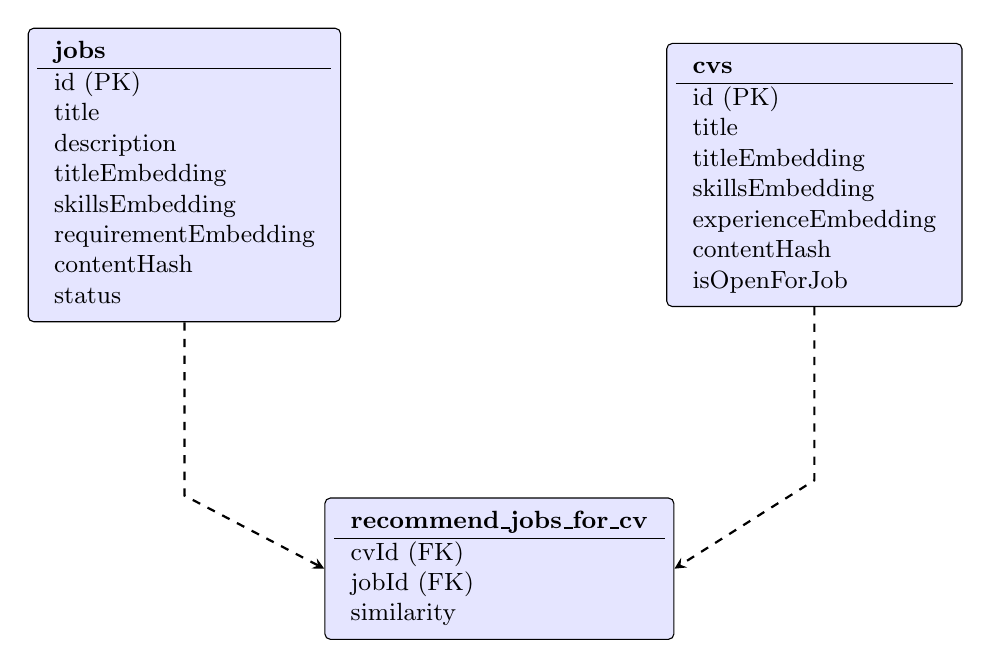
\begin{tikzpicture}[
    table/.style={rectangle, draw, fill=blue!10, minimum width=3.5cm, text centered, font=\small, rounded corners=2pt},
    subtable/.style={rectangle, draw, fill=green!10, minimum width=2.5cm, minimum height=0.6cm, text centered, font=\footnotesize, rounded corners=2pt},
    arrow/.style={->, >=stealth, thick}
]

% Job entity
\node[table] (job) at (-4, 2) {
\begin{tabular}{l}
\textbf{jobs} \\
\hline
id (PK) \\
title \\
description \\
titleEmbedding \\
skillsEmbedding \\
requirementEmbedding \\
contentHash \\
status \\
\end{tabular}
};

% Job sub-tables
% \node[subtable] (jobskill) at (-7, -1) {job\_skills};
% \node[subtable] (jobreq) at (-4, -1) {job\_requirements};
% \node[subtable] (jobbenefit) at (-1, -1) {job\_benefits};

% CV entity
\node[table] (cv) at (4, 2) {
\begin{tabular}{l}
\textbf{cvs} \\
\hline
id (PK) \\
title \\
titleEmbedding \\
skillsEmbedding \\
experienceEmbedding \\
contentHash \\
isOpenForJob \\
\end{tabular}
};

% CV sub-tables
% \node[subtable] (cvskill) at (1.5, -1) {cv\_skills};
% \node[subtable] (workexp) at (4, -1) {work\_experiences};
% \node[subtable] (edu) at (6.5, -1) {educations};

% Recommendation table
\node[table] (rec) at (0, -3) {
\begin{tabular}{l}
\textbf{recommend\_jobs\_for\_cv} \\
\hline
cvId (FK) \\
jobId (FK) \\
similarity \\
\end{tabular}
};

% % Arrows from Job
% \draw[arrow] (job) -- (jobskill);
% \draw[arrow] (job) -- (jobreq);
% \draw[arrow] (job) -- (jobbenefit);

% % Arrows from CV
% \draw[arrow] (cv) -- (cvskill);
% \draw[arrow] (cv) -- (workexp);
% \draw[arrow] (cv) -- (edu);

% Arrows to recommendation
\draw[arrow, dashed] (job.south) -- ++(0,-2.2) -- (rec.west);
\draw[arrow, dashed] (cv.south) -- ++(0,-2.2) -- (rec.east);

\end{tikzpicture}
\caption{Lược đồ cơ sở dữ liệu hệ thống gợi ý}
\label{fig:db-schema}
\end{figure} 

Khi tính vector nhúng, hệ thống truy vấn dữ liệu từ các bảng quan hệ và ghép nối thành văn bản đầu vào cho mô hình. Ví dụ, để tính skillsEmbedding của một công việc, hệ thống lấy tất cả bản ghi từ bảng job\_skills có jobId tương ứng, ghép các tên kỹ năng thành chuỗi văn bản, rồi đưa qua mô hình SimCSE để có vector 768 chiều. Vector nhúng được lưu dưới dạng JSON trong bảng chính để tiện truy xuất khi cần.

\begin{table}[H]
\centering
\caption{Các trường vector nhúng trong cơ sở dữ liệu}
\label{tab:embedding-fields}
\begin{tabular}{|l|l|l|}
\hline
\textbf{Bảng} & \textbf{Trường} & \textbf{Nguồn dữ liệu} \\
\hline
\multirow{3}{*}{jobs} & titleEmbedding & Tiêu đề công việc \\
\cline{2-3}
& skillsEmbedding & Ghép nối từ bảng job\_skills \\
\cline{2-3}
& requirementEmbedding & Ghép nối từ bảng job\_requirements \\
\hline
\multirow{3}{*}{cvs} & titleEmbedding & Tiêu đề mong muốn \\
\cline{2-3}
& skillsEmbedding & Ghép nối từ bảng cv\_skills \\
\cline{2-3}
& experienceEmbedding & Ghép nối từ bảng work\_experiences \\
\hline
\end{tabular}
\end{table}

\subsubsection{Chỉ mục FAISS}

FAISS index được xây dựng từ các vector tiêu đề công việc trong PostgreSQL để phục vụ vòng lọc đầu tiên của thuật toán lọc phân tầng. Hệ thống sử dụng loại index IVFFlat với cấu hình phù hợp cho quy mô dữ liệu hiện tại.

\begin{table}[H]
\centering
\caption{Cấu hình FAISS index}
\label{tab:faiss-config}
\begin{tabular}{|l|l|l|}
\hline
\textbf{Tham số} & \textbf{Giá trị} & \textbf{Mô tả} \\
\hline
Index type & IVFFlat & Tìm kiếm láng giềng gần đúng dựa trên phân cụm \\
\hline
Số chiều & 768 & Tương ứng với đầu ra PhoBERT \\
\hline
nlist & 100 & Số lượng cụm trong index \\
\hline
nprobe & 10 & Số cụm được tìm kiếm khi truy vấn \\
\hline
\end{tabular}
\end{table}

Chiến lược lưu trữ kép được áp dụng trong đó PostgreSQL đóng vai trò nguồn dữ liệu chính đảm bảo tính bền vững, còn FAISS index được tải vào bộ nhớ RAM để tối ưu tốc độ truy vấn. Chỉ mục FAISS được lưu xuống đĩa dưới dạng file với đuôi \texttt{.faiss} để tránh phải xây dựng lại sau mỗi lần khởi động lại dịch vụ.

\subsection{Luồng truy vấn}
\label{subsec:luong-truy-van}

\subsubsection{Quy trình gợi ý CV-Job}

Quy trình gợi ý việc làm cho CV được thực hiện qua năm bước chính. Bước một, hệ thống tải danh sách CV và công việc từ PostgreSQL với các vector nhúng đã được tính toán trước. Bước hai, kiểm tra mã băm nội dung để xác định các bản ghi có nội dung thay đổi và chỉ tính lại vector nhúng cho những bản ghi này. Bước ba, xây dựng hoặc tải chỉ mục FAISS từ các vector tiêu đề công việc. Bước bốn, áp dụng thuật toán lọc phân tầng ba vòng để tìm $K_3$ công việc phù hợp nhất cho mỗi CV. Bước năm, lưu kết quả gợi ý vào bảng RecommendJobForCV.

\subsubsection{Thuật toán lọc phân tầng}

Thuật toán lọc phân tầng sử dụng ba vòng lọc tuần tự để thu hẹp dần tập ứng viên từ toàn bộ công việc xuống còn $K_3$ kết quả cuối cùng. Hình \ref{fig:cascade-flow} minh họa luồng xử lý của thuật toán với các tham số cấu hình $K_1$, $K_2$, $K_3$ tương ứng cho từng vòng.

\begin{figure}[H]
\centering
\begin{tikzpicture}[
    stage/.style={rectangle, draw, fill=blue!10, minimum width=4cm, minimum height=1cm, text centered, font=\small, rounded corners=3pt},
    count/.style={rectangle, fill=gray!20, minimum width=2cm, minimum height=0.6cm, text centered, font=\footnotesize},
    arrow/.style={->, >=stealth, thick}
]

\node[count] (n0) at (0, 4) {$N$ Jobs};
\node[stage] (s1) at (0, 3) {Vòng 1: Lọc theo tiêu đề (FAISS)};
\node[count] (n1) at (0, 2) {$K_1$ Jobs};
\node[stage] (s2) at (0, 1) {Vòng 2: Lọc theo kinh nghiệm};
\node[count] (n2) at (0, 0) {$K_2$ Jobs};
\node[stage] (s3) at (0, -1) {Vòng 3: Lọc theo kỹ năng};
\node[count] (n3) at (0, -2) {$K_3$ Jobs};

\draw[arrow] (n0) -- (s1);
\draw[arrow] (s1) -- (n1);
\draw[arrow] (n1) -- (s2);
\draw[arrow] (s2) -- (n2);
\draw[arrow] (n2) -- (s3);
\draw[arrow] (s3) -- (n3);

\end{tikzpicture}
\caption{Luồng xử lý thuật toán lọc phân tầng}
\label{fig:cascade-flow}
\end{figure}

Các tham số $K_1$, $K_2$, $K_3$ được cấu hình qua biến môi trường, với giá trị mặc định lần lượt là 1000, 300 và 30. Việc tách riêng các tham số này cho phép điều chỉnh linh hoạt tùy theo quy mô dữ liệu và yêu cầu về độ chính xác.

\textbf{Vòng 1 - Lọc theo tiêu đề.} Vòng đầu tiên sử dụng chỉ mục FAISS để tìm $K_1$ công việc có tiêu đề tương đồng nhất với tiêu đề mong muốn của CV. Vector tiêu đề CV được chuẩn hóa L2 và truy vấn trên chỉ mục FAISS sử dụng độ tương đồng cosin. Việc sử dụng FAISS với index IVFFlat ở vòng này giúp giảm khối lượng tính toán bằng cách chỉ tìm kiếm trong một số cụm gần nhất thay vì toàn bộ tập dữ liệu.

\textbf{Vòng 2 - Lọc theo kinh nghiệm.} Vòng thứ hai so sánh vector kinh nghiệm của CV với vector yêu cầu của $K_1$ công việc từ vòng trước để chọn ra $K_2$ công việc có độ khớp cao nhất. Việc tính toán được thực hiện bằng vòng lặp trực tiếp thay vì xây dựng chỉ mục FAISS mới vì với $K_1$ phần tử, chi phí xây dựng chỉ mục lớn hơn chi phí tính toán trực tiếp. Đối với CV không có kinh nghiệm như sinh viên mới ra trường, hệ thống áp dụng chiến lược bỏ qua vòng lọc này (skip layer) và giữ nguyên tất cả $K_1$ công việc từ vòng trước, đảm bảo các ứng viên mới vẫn được xếp hạng công bằng dựa trên độ tương đồng tiêu đề và kỹ năng.

\textbf{Vòng 3 - Lọc theo kỹ năng.} Vòng cuối cùng so sánh vector kỹ năng của CV với vector kỹ năng của $K_2$ công việc từ vòng trước để chọn ra $K_3$ kết quả cuối cùng. Tương tự vòng 2, nếu CV không có thông tin kỹ năng, vòng lọc này được bỏ qua.

Bảng \ref{tab:cascade-complexity} tổng hợp độ phức tạp của từng vòng lọc, trong đó $d$ là số chiều của vector nhúng (768 chiều).

\begin{table}[H]
\centering
\caption{Độ phức tạp thuật toán lọc phân tầng}
\label{tab:cascade-complexity}
\begin{tabular}{|l|l|l|l|}
\hline
\textbf{Vòng} & \textbf{Đầu vào} & \textbf{Đầu ra} & \textbf{Độ phức tạp} \\
\hline
1 - Tiêu đề (FAISS IVF) & $N$ & $K_1$ & $O\left(\frac{N \cdot \text{nprobe}}{\text{nlist}} \cdot d\right)$ \\
\hline
2 - Kinh nghiệm & $K_1$ & $K_2$ & $O(K_1 \cdot d)$ \\
\hline
3 - Kỹ năng & $K_2$ & $K_3$ & $O(K_2 \cdot d)$ \\
\hline
\end{tabular}
\end{table}

Với cấu hình FAISS sử dụng $\text{nlist} = 100$ và $\text{nprobe} = 10$, vòng 1 chỉ cần tìm kiếm trong khoảng 10\% số cụm thay vì toàn bộ tập dữ liệu. So với phương pháp vét cạn tính độ tương đồng giữa một CV với tất cả công việc cần $O(3 \cdot N \cdot d)$ phép tính, thuật toán lọc phân tầng giảm đáng kể khối lượng tính toán nhờ thu hẹp dần không gian tìm kiếm qua từng vòng.

\subsection{Tối ưu hóa}
\label{subsec:toi-uu-hoa}

Hệ thống áp dụng nhiều chiến lược tối ưu hóa để giảm thời gian xử lý và tài nguyên tính toán. 

\subsubsection{Bộ nhớ đệm mã băm nội dung}

Việc tính toán vector nhúng qua mô hình ngôn ngữ là tác vụ tốn kém tài nguyên, đặc biệt khi xử lý hàng nghìn bản ghi. Để tránh tính toán lại khi nội dung không thay đổi, hệ thống sử dụng cơ chế mã băm nội dung. Hình \ref{fig:content-hash-flow} minh họa luồng xử lý của cơ chế này.

\begin{figure}[H]
\centering
\begin{tikzpicture}[
    process/.style={rectangle, draw, fill=blue!10, minimum width=3cm, minimum height=0.8cm, text centered, font=\small, rounded corners=2pt},
    decision/.style={diamond, draw, fill=yellow!20, minimum width=2cm, minimum height=1cm, text centered, font=\small, aspect=2},
    data/.style={rectangle, draw, fill=green!10, minimum width=2.5cm, minimum height=0.6cm, text centered, font=\footnotesize, rounded corners=2pt},
    arrow/.style={->, >=stealth, thick}
]

% Flow
\node[process] (load) at (0, 4) {Tải bản ghi từ DB};
\node[process] (compute) at (0, 2.5) {Tính mã băm mới};
\node[decision] (check) at (0, 1) {Hash khác?};
\node[process] (embed) at (-3, -0.5) {Tính embedding mới};
\node[process] (skip) at (3, -0.5) {Giữ embedding cũ};
\node[process] (save) at (-3, -2) {Lưu vào DB};
\node[process] (next) at (0, -3) {Xử lý bản ghi tiếp};

% Arrows
\draw[arrow] (load) -- (compute);
\draw[arrow] (compute) -- (check);
\draw[arrow] (check) -- node[left, font=\footnotesize] {Có} (-3, 1) -- (embed);
\draw[arrow] (check) -- node[right, font=\footnotesize] {Không} (3, 1) -- (skip);
\draw[arrow] (embed) -- (save);
\draw[arrow] (save) -- (next);
\draw[arrow] (skip) -- (3, -3) -- (next);

% Hash computation detail
\node[data] (detail) at (5, 2.5) {title + skills + experience};
\draw[arrow, dashed] (detail) -- (compute);

\end{tikzpicture}
\caption{Luồng xử lý bộ nhớ đệm mã băm nội dung}
\label{fig:content-hash-flow}
\end{figure}

Với mỗi bản ghi, mã băm được tính từ các trường thông tin dùng để tạo embedding. Đối với công việc, mã băm được tính theo công thức:
\begin{equation}
h_{job} = \text{MD5}\left(\text{JSON}\left(\{\text{title}, \text{skills}, \text{requirements}\}\right)\right)
\end{equation}

Tương tự, đối với CV:
\begin{equation}
h_{cv} = \text{MD5}\left(\text{JSON}\left(\{\text{title}, \text{currentPosition}, \text{skills}, \text{experiences}\}\right)\right)
\end{equation}

Quá trình xử lý cho mỗi bản ghi được thực hiện như sau. Đầu tiên, hệ thống truy vấn dữ liệu từ các bảng quan hệ bao gồm bảng chính và các bảng kỹ năng, kinh nghiệm. Tiếp theo, mã băm mới được tính từ nội dung hiện tại bằng cách chuyển đổi các trường sang định dạng JSON và áp dụng hàm băm MD5. Sau đó, mã băm mới được so sánh với mã băm đã lưu trong cơ sở dữ liệu. Nếu hai mã băm khác nhau hoặc bản ghi chưa có embedding, hệ thống tính toán embedding mới và cập nhật cả embedding lẫn mã băm vào cơ sở dữ liệu. Nếu hai mã băm giống nhau, bản ghi được bỏ qua để tiết kiệm thời gian.

Cơ chế này đặc biệt hiệu quả vì trong thực tế, phần lớn dữ liệu không thay đổi giữa các lần cập nhật. Ví dụ, nếu chỉ có 5\% bản ghi thay đổi, hệ thống chỉ cần tính toán embedding cho 5\% đó thay vì toàn bộ tập dữ liệu, giảm đáng kể thời gian xử lý.

\subsubsection{Lọc công việc đang hoạt động}

Hệ thống chỉ xử lý các công việc thỏa mãn điều kiện đang hoạt động thay vì toàn bộ công việc trong cơ sở dữ liệu. Điều kiện lọc bao gồm trạng thái công việc phải là ACTIVE và thời hạn hết hạn chưa qua hoặc không được đặt. Điều kiện này được thể hiện trong mệnh đề WHERE của truy vấn SQL như sau:

\begin{lstlisting}[language=SQL, basicstyle=\ttfamily\small, frame=single, breaklines=true]
SELECT j.* FROM jobs j
WHERE j.status = 'ACTIVE'
  AND (j."expiresAt" IS NULL OR j."expiresAt" > NOW())
\end{lstlisting}

Chiến lược này mang lại hai lợi ích. Thứ nhất, giảm khối lượng tính toán vì không cần xử lý các công việc đã đóng hoặc hết hạn. Thứ hai, đảm bảo kết quả gợi ý chỉ bao gồm các cơ hội việc làm còn hiệu lực, nâng cao trải nghiệm người dùng.

\subsubsection{Cập nhật định kỳ}

Hệ thống thực hiện tác vụ cập nhật định kỳ để đảm bảo kết quả gợi ý phản ánh dữ liệu mới nhất. Chu kỳ cập nhật được cấu hình qua biến môi trường với giá trị mặc định 12 giờ. Hình \ref{fig:update-pipeline} minh họa quy trình cập nhật định kỳ.

\begin{figure}[H]
\centering
\begin{tikzpicture}[
    process/.style={rectangle, draw, fill=blue!10, minimum width=3.5cm, minimum height=0.8cm, text centered, font=\small, rounded corners=2pt},
    check/.style={rectangle, draw, fill=yellow!20, minimum width=3.5cm, minimum height=0.8cm, text centered, font=\small, rounded corners=2pt},
    arrow/.style={->, >=stealth, thick}
]

% Pipeline steps
\node[process] (step1) at (0, 4) {1. Tải công việc đang hoạt động};
\node[check] (step2) at (0, 3) {2. Kiểm tra mã băm, cập nhật embedding};
\node[process] (step3) at (0, 2) {3. Tải CV chính};
\node[check] (step4) at (0, 1) {4. Kiểm tra mã băm, cập nhật embedding};
\node[process] (step5) at (0, 0) {5. Tải/xây dựng chỉ mục FAISS};
\node[process] (step6) at (0, -1) {6. Chạy thuật toán lọc phân tầng};
\node[process] (step7) at (0, -2) {7. Lưu kết quả gợi ý};

% Arrows
\draw[arrow] (step1) -- (step2);
\draw[arrow] (step2) -- (step3);
\draw[arrow] (step3) -- (step4);
\draw[arrow] (step4) -- (step5);
\draw[arrow] (step5) -- (step6);
\draw[arrow] (step6) -- (step7);

% Side notes
\node[font=\footnotesize, text=gray, align=left] at (4.5, 3.5) {Lọc status='ACTIVE'\\và chưa hết hạn};
\node[font=\footnotesize, text=gray, align=left] at (4.5, 0.5) {Chỉ cập nhật\\bản ghi thay đổi};
\node[font=\footnotesize, text=gray, align=left] at (4.5, -1.5) {Xóa gợi ý cũ\\trước khi lưu mới};

\end{tikzpicture}
\caption{Quy trình cập nhật định kỳ}
\label{fig:update-pipeline}
\end{figure}

Quy trình cập nhật bao gồm bảy bước chính. Bước một, tải danh sách công việc đang hoạt động từ cơ sở dữ liệu với điều kiện lọc phù hợp. Bước hai, với mỗi công việc, kiểm tra mã băm nội dung và chỉ tính lại embedding cho những công việc có nội dung thay đổi. Bước ba, tải danh sách CV chính của người dùng. Bước bốn, tương tự bước hai, kiểm tra và cập nhật embedding cho các CV có nội dung thay đổi. Bước năm, tải chỉ mục FAISS đã lưu hoặc xây dựng mới nếu cần. Bước sáu, chạy thuật toán lọc phân tầng để tìm công việc phù hợp cho mỗi CV. Bước bảy, lưu kết quả gợi ý vào cơ sở dữ liệu, xóa các gợi ý cũ trước khi lưu gợi ý mới.

Chu kỳ 12 giờ được lựa chọn để cân bằng giữa độ tươi mới của dữ liệu và tải hệ thống. Trong trường hợp cần cập nhật nhanh hơn, chu kỳ có thể được điều chỉnh qua biến môi trường mà không cần thay đổi mã nguồn.

